\documentclass[12pt]{article}
\setlength{\oddsidemargin}{0in}
\setlength{\evensidemargin}{0in}
\setlength{\textwidth}{6.5in}
\setlength{\parindent}{0in}
\setlength{\parskip}{\baselineskip}

\usepackage{amsmath,amsfonts,amssymb,bm,graphics,pgfplots,framed,dsfont}
\usepackage[scale=0.75,top=1cm,bottom=3cm]{geometry}

\begin{document}

\textbf{Minh Anh Nguyen }\\
\textbf{Calculus 1 Assignment-7}\\
\textbf{Section: 04}\\
\textbf{TA's name: Arthur Huey}

\hrulefill

Section 3.4:

\begin{enumerate}
    \setcounter{enumi}{2}
    \item For the function $f$ whose graph is given, state the following.
    \begin{center}
        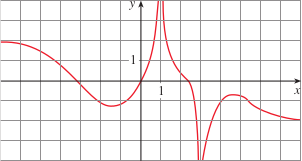
\includegraphics{img/img-0.png}
    \end{center}
    \begin{enumerate}
        \item \[\boxed{\lim_{x \to \infty } f(x) = -2}\]
        \item \[\boxed{\lim_{x \to -\infty} f(x) = 2}\]
        \item \[\boxed{\lim_{x \to 1} f(x) = \infty}\]
        \item \[\boxed{\lim_{x \to 3} f(x) = -\infty}\]
        \item The equations of the asymptotes
        \[\boxed{x = 1, x = 3, y = -2, y = 2}\]
    \end{enumerate}
    \setcounter{enumi}{7}
    \item Evaluate the limit and justify each step by indicating the appropriate properties of limits.
    \[\lim_{x \to \infty} \sqrt{\frac{9x^3+8x-4}{3-5x+x^3}}\]
    \[= \lim_{x \to \infty} \sqrt{\frac{x^3(9+8/x^2-4/x^3)}{x^3(3/x^3-5/x^2+1)}}\]
    \[= \lim_{x \to \infty} \sqrt{\frac{9+8/x^2-4/x^3}{3/x^3-5/x^2+1}}\]
    \[= \sqrt{\frac{9+0-0}{0-0+1}}\]
    \[\boxed{= \sqrt{9} = 3}\]
    \setcounter{enumi}{10}
    \item Find the limit or show that it does not exist.
    \[\lim_{t \to -\infty} \frac{3t^2 + t}{t^3 -4t + 1}\]
    \[= \lim_{t \to -\infty} \frac{t^2(3 + 1/t)}{t^3(1 -4/t^2 + 1/t^3)}\]
    \[= \lim_{t \to -\infty} \frac{(3 + 1/t)}{t(1 -4/t^2 + 1/t^3)}\]
    \[\boxed{= 0}\]
    \setcounter{enumi}{17}
    \item Find the limit or show that it does not exist.
    \[\lim_{t \to \infty}\frac{t+3}{\sqrt{2t^2-1}}\]
    \[=\lim_{t \to \infty}\frac{t(1+3/t)}{t\sqrt{2-1/t^2}}\]
    \[=\lim_{t \to \infty}\frac{1+3/t}{\sqrt{2-1/t^2}}\]
    \[=\frac{1+0}{\sqrt{2-0}}\]
    \[\boxed{=\frac{1}{\sqrt{2}}}\]
    \setcounter{enumi}{25}
    \item Find the limit or show that it does not exist.
    \[=\lim_{x \to -\infty}(\sqrt{4x^2 + 3x} + 2x)\]
    \[=\lim_{x \to -\infty}(|x|\sqrt{4 + 3/x} + 2x)\]
    Because $x$ is approaching to $-\infty$. $|x| = -x$.
    \[=\lim_{x \to -\infty}(-x\sqrt{4 + 3/x} + 2x)\]
    \[=\lim_{x \to -\infty}x(-\sqrt{4 + 3/x} + 2)\]
    \[=-\infty(-2 + 2)\]
    \[=-\infty(0)\]
    \[\boxed{=0}\]
    \newpage
    \setcounter{enumi}{27}
    \item Find the limit or show that it does not exist.
    \[\lim_{x \to \infty}(x - \sqrt{x})\]
    \[=\lim_{x \to \infty}x(1 - 1/\sqrt{x})\]
    \[=\infty(1 - 0)\]
    \[\boxed{=\infty}\]
    \setcounter{enumi}{30}
    \item Find the limit or show that it does not exist.
    \[\lim_{x\to \infty}x\sin\frac{1}{x}\]
    \[=\infty\sin 0\]
    \[\boxed{=0}\]
    \setcounter{enumi}{36}
    \item Find the horizontal and vertical asymptotes of each curve. You may want to use a graphing calculator (or computer) to check your work by graphing the curve and estimating the asymptotes.
    \[y = \frac{2x^2 + x - 1}{x^2 + x - 2}\]
    Horizontal Asymptotes:
    \[\lim_{x\to \infty}\frac{2x^2 + x - 1}{x^2 + x - 2}\]
    \[=\lim_{x\to \infty}\frac{x^2(2 + 1/x - 1/x^2)}{x^2(1 + 1/x - 2/x^2)}\]
    \[=\lim_{x\to \infty}\frac{2 + 1/x - 1/x^2}{1 + 1/x - 2/x^2}\]
    \[\boxed{=2}\]
    \[\lim_{x\to -\infty}\frac{2x^2 + x - 1}{x^2 + x - 2}\]
    \[=\lim_{x\to -\infty}\frac{x^2(2 + 1/x - 1/x^2)}{x^2(1 + 1/x - 2/x^2)}\]
    \[=\lim_{x\to -\infty}\frac{2 + 1/x - 1/x^2}{1 + 1/x - 2/x^2}\]
    \[\boxed{=2}\]
    \[\boxed{y = 2}\]
    Vertical Asymptotes;
    \[x^2 + x - 2 = 0\]
    \[(x-1)(x+2) = 0\]
    \[\boxed{x=1\text{ or }x=-2}\]
    \[\boxed{x = 1, x = -2}\]
    \newpage
    \setcounter{enumi}{53}
    \item Find the limits as $x \to \infty$ and as $x \to -\infty$. Use this information, together with intercepts, to give a rough sketch of the graph as in Example 11.
    \[y = x^3(x + 2)^2(x-1)\]
    \[\lim_{x\to \infty}x^3(x + 2)^2(x-1)\]
    \[\boxed{=\infty}\]
    ~\\~
    \[\lim_{x\to -\infty}x^3(x + 2)^2(x-1)\]
    \[\boxed{= -\infty}\]
    \begin{figure}[!h]      
        \begin{framed}
            \centering  
            \begin{tikzpicture}
                \begin{axis}[
                    axis lines = middle,
                    xlabel = $x$,
                    ylabel = {$f(x)$},
                    samples = 100,
                    domain = -4:2,
                    ymin=-10, ymax=10,
                ]
                \addplot[
                    thick,
                    blue,
                ]{x^3*(x + 2)^2*(x - 1)};
                \end{axis}
            \end{tikzpicture}
        \end{framed}
        \end{figure}
    \setcounter{enumi}{58}
    \item Sketch the graph of a function that satisfies all of the given conditions.
\end{enumerate}
\newpage
Section 3.5:
\begin{enumerate}
\setcounter{enumi}{4}
    \item Use the guidelines of this section to sketch the curve.
    \[y = x(x-4)^3\]
\end{enumerate}

\end{document}